\documentclass[conference]{IEEEtran}
\IEEEoverridecommandlockouts
\usepackage{cite}
\usepackage{amsmath,amssymb,amsfonts}
\usepackage{mathtools}
\usepackage{algorithmic}
\usepackage{graphicx}
\usepackage{booktabs}
\usepackage{textcomp}
\usepackage{xcolor}
\usepackage{url}
\usepackage{dblfloatfix}
\usepackage{placeins}
\allowdisplaybreaks[1]
\setcounter{topnumber}{3}
\setcounter{dbltopnumber}{2}
\setcounter{totalnumber}{4}
\renewcommand{\topfraction}{0.95}
\renewcommand{\dbltopfraction}{0.95}
\renewcommand{\textfraction}{0.05}
\renewcommand{\floatpagefraction}{0.80}
\renewcommand{\dblfloatpagefraction}{0.80}
\setlength{\textfloatsep}{10pt plus 2pt minus 2pt}
\setlength{\dbltextfloatsep}{10pt plus 2pt minus 2pt}
\setlength{\floatsep}{9pt plus 2pt minus 2pt}
\makeatletter
\setlength{\@fptop}{0pt}
\setlength{\@fpsep}{10pt}
\setlength{\@fpbot}{0pt plus 1fil}
\makeatother
\DeclareMathOperator*{\argmin}{arg\,min}
\def\BibTeX{{\rm B\kern-.05em{\sc i\kern-.025em b}\kern-.08em
T\kern-.1667em\lower.7ex\hbox{E}\kern-.125emX}}

\title{RouteCast: Calibrated Cross-Token Expert Forecasting with Selective Cache-Aware Prefetching for Heterogeneous MoE Models}

\author{\IEEEauthorblockN{Jihua Dong}
\IEEEauthorblockA{\textit{School of Microelectronics} \\
\textit{University of Electronic Science and Technology of China}\\
Chengdu, China \\
2023190903038@std.uestc.edu.cn}}

\begin{document}
\maketitle
\begin{abstract}
Sparse mixture-of-experts (MoE) inference may place expert-weight transfers on
the critical path when selected experts are not resident in accelerator memory.
Prefetching can hide these transfers, but inaccurate predictions increase data
movement and pollute limited expert caches. We present RouteCast, a route-only
framework that couples expert forecasting with selective prefetching. A
context-conditioned gate integrates six complementary evidence branches:
global popularity, one-step transitions, two-hop transitions, request-level
prefill statistics, recurrent routing history, and multiscale temporal
context. RouteCast calibrates the resulting scores, adapts the candidate
budget to prediction confidence, and admits only candidates expected to benefit
the cache. The framework requires neither hidden states nor modifications to
the native router.

We evaluate RouteCast using request-disjoint traces comprising 1,000 requests
from each of three heterogeneous MoE architectures: Qwen3, DeepSeek-R1, and
Llama4 Maverick. Under their native expert budgets, RouteCast achieves Recall
values of 0.5558, 0.3172, and 0.3602, respectively. These results exceed
matched temporal convolutional network (TCN) predictors by 2.81, 4.55, and
5.79 percentage points, corresponding to relative improvements of 5.3\%,
16.7\%, and 19.1\%. RouteCast also consistently outperforms paper-derived and
request-aware heatmap baselines across the three routing regimes. Confidence
intervals from 10,000 paired request-level bootstrap resamples exclude zero
for all three RouteCast--TCN comparisons. Component ablations further show
that recurrent routing history and context-conditioned multi-source fusion
provide complementary gains. Budget sweeps reveal explicit trade-offs between
expert coverage and transfer volume, while trace-driven cache replay shows
that selective admission reduces unnecessary transfers relative to unfiltered
adaptive prefetching. Together, these results establish RouteCast as a
calibrated interface between route prediction and budget-aware expert
prefetching. The present trace-based evaluation does not establish
end-to-end latency improvements in a deployed MoE system.
\end{abstract}


\begin{IEEEkeywords}
sparse mixture-of-experts, route-only prediction, expert prefetching,
confidence calibration, adaptive candidate budget, cache-aware scheduling
\end{IEEEkeywords}

\section{Introduction}
Sparse mixture-of-experts (MoE) language models increase parameter capacity
while activating only a small subset of experts for each token. This
conditional computation reduces arithmetic cost, but the complete expert pool
may still exceed accelerator memory. In an offloaded deployment, an expert
that is not resident must be transferred from host memory or another device
after it is selected by the native router. Because this transfer occurs
between routing and expert execution, reactive loading can expose
data-movement latency on the inference critical path.

Speculative expert prefetching attempts to transfer likely experts before they
are requested. Previous studies have explored router co-design, proactive
expert movement, and sparsity-aware caching
\cite{pregated,moeinfinity,promoe}. Public route traces further indicate that
expert selections exhibit exploitable spatial and temporal structure
\cite{patterns}. Prediction recall alone, however, is insufficient. Enlarging
the candidate set can trivially cover more true experts, but it also increases
false transfers, cache pollution, and replacement pressure. A practical
prefetching method must therefore address three coupled questions: which
experts are likely to be selected, how reliable are the predicted scores, and
which predictions should be converted into physical transfers under a finite
cache budget?

We study these questions under a route-only constraint. RouteCast observes
discrete expert identifiers from earlier token positions together with
structural metadata, but it does not access hidden activations or
native-router logits. This constraint makes the predictor applicable when
route traces are available but modifying the serving model is undesirable. It
also creates a difficult forecasting problem across heterogeneous routing
regimes. Qwen3 and DeepSeek-R1 select eight experts from model-specific expert
pools, whereas Llama4 Maverick selects a single expert. Consequently, a fixed
heuristic or a predictor tuned to one architecture may not transfer reliably
to another.

\begin{figure*}[!t]
\centering
\includegraphics[width=0.98\textwidth]{figures_final/Fig1_Framework}
\caption{RouteCast pipeline for route-only expert forecasting and selective
prefetching.}
\label{fig:framework}
\end{figure*}

Figure~\ref{fig:framework} presents the complete RouteCast pipeline. Historical
expert routes are first transformed into six complementary evidence streams:
global popularity, one-step transitions, two-hop transitions, request-level
prefill statistics, recurrent temporal history, and multiscale routing
context. Each branch produces a distribution of scores over the expert pool
rather than an independent hard decision. A context-conditioned
probability-mixture gate assigns input-dependent weights to the six
distributions and produces a fused expert ranking. Model-specific temperature
scaling then converts the fused scores into calibrated probabilities.

The calibrated distribution provides an interface between prediction and
prefetch action. Given a probability-mass threshold, RouteCast selects the
smallest ranked expert prefix whose cumulative probability reaches that
threshold. This mechanism adapts the candidate width to the concentration of
the predicted distribution instead of applying a fixed prefetch width to every
token. Confidence rejection suppresses low-utility predictions, while
cache-aware admission determines which remaining candidates should trigger
physical transfers. The native router remains authoritative for execution;
RouteCast only predicts future selections and proposes speculative prefetch
actions.

This design separates three concerns that are often evaluated independently:
expert ranking, confidence estimation, and resource-aware action. The
forecasting stage determines which experts are likely to be selected.
Calibration makes score distributions comparable and supports meaningful
probability-mass decisions. Selective admission then limits the transfer and
cache costs caused by incorrect predictions. This separation also allows
prediction quality to be evaluated independently from cache-replay outcomes,
preventing improvements obtained solely by enlarging the prefetch budget from
being mistaken for better forecasting.

The study makes three contributions:

\begin{itemize}
    \item We establish a request-disjoint protocol for next-token expert
    forecasting across three heterogeneous public MoE trace families. The
    protocol preserves model-specific native expert budgets and reports
    ranking quality under matched train, validation, and test partitions.

    \item We introduce a route-only predictor that combines four statistical
    priors with recurrent and multiscale temporal evidence through a
    context-conditioned probability-mixture gate. The predictor requires
    neither hidden states nor modifications to the native router.

    \item We connect calibrated expert prediction to adaptive candidate
    selection, confidence rejection, and cache-aware admission. Budget sweeps,
    component ablations, request-level bootstrap analysis, and trace-driven
    cache replay jointly characterize prediction gains, transfer trade-offs,
    and model--capacity failure boundaries.
\end{itemize}

The resulting evidence is algorithmic and trace-driven. It establishes the
quality of route forecasting and selective prefetch decisions, but it does not
demonstrate end-to-end latency, throughput, or energy improvements in a
deployed MoE serving system.


\section{Related Work}

\textbf{MoE inference and expert movement.}
Memory-constrained MoE inference commonly places inactive experts in host
memory or secondary storage and transfers them to the accelerator on demand.
Pre-gated MoE co-designs expert selection and execution to overlap expert
movement with useful computation \cite{pregated}. MoE-Infinity exploits
activation sparsity through a sparsity-aware expert cache on
memory-constrained machines \cite{moeinfinity}, whereas ProMoE investigates
proactive expert caching for MoE serving \cite{promoe}. These studies
demonstrate that expert movement can be hidden or avoided through prediction,
caching, and execution overlap. Their end-to-end gains, however, necessarily
depend on deployment-specific factors such as cache capacity, transfer
bandwidth, scheduling policy, and available computation overlap. RouteCast
focuses on the complementary problem of producing calibrated expert forecasts
before those predictions are consumed by a particular runtime.

\textbf{Expert-route forecasting.}
\emph{Patterns behind Chaos} identifies spatial and temporal regularities in
expert-selection traces and provides the public trace data used in this study
\cite{patterns}. Related spatio-temporal predictors exploit dependencies
across tokens or layers to estimate future expert selections \cite{stmoe}.
These observations establish that historical routes contain predictive
information, but the usefulness of each dependency can vary across models,
requests, layers, and routing regimes. RouteCast therefore treats route
statistics as conditionally informative evidence rather than applying a fixed
fusion rule. Its context-conditioned gate combines normalized distributions
from global popularity, one-step transitions, two-hop transitions,
request-level prefill statistics, recurrent history, and multiscale temporal
context. This design also preserves the route-only constraint: no hidden
activations or native-router logits are required.

\textbf{From prediction to prefetch action.}
Recent speculative prefetching methods increasingly recognize that a correct
ranking is useful only when candidate transfers can be issued early and
without excessive cache disruption \cite{specmd,specprefetch}. This distinction
is important because increasing the prefetch width can improve expert coverage
while simultaneously increasing false transfers and cache pollution.
RouteCast makes the distinction explicit by separating forecasting, candidate
selection, and cache action. Fixed-budget Recall and ranking metrics evaluate
the forecaster independently of resource decisions. Temperature calibration
and adaptive probability mass determine the candidate interface, while
confidence rejection and cache-aware admission decide which candidates become
physical prefetch requests. Trace-driven cache replay then measures cache hit
rate, transfer volume, and wasted prefetches. This layered evaluation prevents
an increase in expert coverage from being interpreted as an equivalent
end-to-end system speedup.

\section{RouteCast Design}
\subsection{Problem Formulation and Design Principles}

For request $r$, token position $t$, and routed layer $\ell$, let $E_r$
denote the number of candidate experts and $K_r$ denote the number selected by
the native router. The routing decision is represented by
$\mathbf{y}_{r,t,\ell}\in\{0,1\}^{E_r}$, where
$\|\mathbf{y}_{r,t,\ell}\|_0=K_r$. Its non-zero entries define the executed
expert set $\mathcal{Y}_{r,t,\ell}$.

RouteCast predicts the expert set at the same routed layer for the next token:
\begin{align}
\mathbf{s}_{r,t+1,\ell}
&=
f_{\theta}\!\left(
\mathcal{R}_{r,\leq t},
\mathbf{c}_{r,t,\ell}
\right), \\
\widehat{\mathcal{Y}}_{r,t+1,\ell}^{(K_r)}
&=
\operatorname{TopK}\!\left(
\mathbf{s}_{r,t+1,\ell},K_r
\right).
\label{eq:task}
\end{align}
Here, $\mathcal{R}_{r,\leq t}$ is the sequence of expert identifiers observed
up to token $t$, and $\mathbf{c}_{r,t,\ell}$ is a five-dimensional structural
context vector. It contains the normalized layer position, expert-pool size,
native routing sparsity, request-prefill entropy, and token position. The
function $f_{\theta}$ denotes the RouteCast predictor with trainable parameters
$\theta$, while $\mathbf{s}_{r,t+1,\ell}\in\mathbb{R}^{E_r}$ contains one
score for each candidate expert. The operator
$\operatorname{TopK}(\cdot,K_r)$ returns the $K_r$ highest-scoring experts.

The prediction problem is heterogeneous across the evaluated traces, as shown
in Table~\ref{tab:route-regimes}. Qwen3 and DeepSeek-R1 share a native routing
width of eight but differ by a factor of two in expert-pool size. Llama4
Maverick instead adopts Top-1 routing and contains substantially fewer routed
layers. The resulting 22.38 million token-layer instances therefore span
different output dimensions, positive-label densities, and temporal routing
structures.

\begin{table}[!t]
\centering
\caption{Routing heterogeneity in the evaluated MoE traces. $E$ denotes the
expert-pool size, $K$ the native routing width, and $L_{\mathrm{MoE}}$ the
number of routed layers.}
\label{tab:route-regimes}
\scriptsize
\setlength{\tabcolsep}{3.2pt}
\begin{tabular}{lrrrr}
\toprule
Model & $E$ & $K$ & $L_{\mathrm{MoE}}$ & Instances \\
\midrule
Qwen3           & 128 & 8 & 94 & 11.96M \\
DeepSeek-R1     & 256 & 8 & 58 &  7.35M \\
Llama4 Maverick & 128 & 1 & 24 &  3.07M \\
\midrule
Total           & --  & -- & -- & 22.38M \\
\bottomrule
\end{tabular}
\end{table}

RouteCast is route-only and causal. It uses neither hidden activations nor
native-router logits, and it observes no information from token $t+1$ when
forming its prediction. The native router remains authoritative: RouteCast may
propose an expert transfer, but it cannot change which experts are executed. A
false positive therefore causes an unnecessary speculative transfer, whereas a
false negative leaves the corresponding demand transfer unhidden.

RouteCast further separates expert ranking from prefetch action:
\begin{align}
\widetilde{\mathbf{p}}_{r,t+1,\ell}
&=
\operatorname{Cal}_{T_r}\!\left(
\mathbf{s}_{r,t+1,\ell}
\right), \\
\mathcal{A}_{r,t+1,\ell}
&=
\pi\!\left(
\widetilde{\mathbf{p}}_{r,t+1,\ell},
\mathcal{C}_{r,t},
m_r,
\tau_r
\right).
\label{eq:decision-stack}
\end{align}
The calibration operator $\operatorname{Cal}_{T_r}$ converts expert scores
into probabilities using the model-specific temperature $T_r$. The policy
$\pi$ receives these probabilities, the current cache state
$\mathcal{C}_{r,t}$, the probability-mass threshold $m_r$, and the confidence
threshold $\tau_r$. It returns the admitted prefetch set
$\mathcal{A}_{r,t+1,\ell}$, which may contain fewer than $K_r$ experts or may
be empty.

This separation allows forecasting quality, candidate coverage, and cache
behavior to be evaluated independently. Forecasting is first evaluated under
the native budget $K_r$, preventing a method from appearing more accurate
merely because it predicts more experts. Adaptive selection is then evaluated
through Recall, Precision, and mean candidate width, while cache replay
measures hit rate, issued transfers, and wasted prefetches. Consequently, an
increase in candidate coverage is not automatically interpreted as an
equivalent improvement in system performance.
\subsection{Multi-Source Route Forecasting}

RouteCast forecasts the expert selection at token \(t+1\) and routed layer
\(\ell\) from routes observed up to token \(t\). Rather than assuming that one
temporal pattern is uniformly reliable, it constructs six complementary
per-expert evidence branches:

\begin{enumerate}
    \item layer-wise global popularity;
    \item one-hop cross-token transition;
    \item two-hop cross-token transition;
    \item request-specific prefill popularity;
    \item recurrent routing history encoded by a GRU; and
    \item multiscale activation frequency and recency.
\end{enumerate}

The first four branches provide statistical priors, while the final two learn
request-local deviations from these priors. All branches produce one score for
each candidate expert, allowing them to be combined by a shared
context-conditioned gate.

\subsubsection{Statistical route evidence}

Let \(E_g\) denote the number of experts in model group \(g\), and let
\(\mathcal{Y}_{t,\ell}\) be the set of experts observed at token \(t\) and
layer \(\ell\). Layer popularity estimates the marginal probability of expert
\(e\) from training requests:

\begin{equation}
q_{\ell,e}^{\mathrm{pop}}
=
\frac{
N_{\ell}^{\mathrm{pop}}(e)
}{
\displaystyle
\sum_{j=1}^{E_g}
N_{\ell}^{\mathrm{pop}}(j)
},
\label{eq:popularity-prior}
\end{equation}

where \(N_{\ell}^{\mathrm{pop}}(e)\) counts how often expert \(e\) is selected
at layer \(\ell\). These statistics are computed exclusively from the
training split.

The one-hop transition branch estimates which experts follow those selected
at the current token. For every source expert
\(u\in\mathcal{Y}_{t,\ell}\), its transition row records the empirical
distribution of experts selected at \(t+1\). The rows associated with all
currently active experts are aggregated and renormalized to obtain

\begin{equation}
\mathbf{q}_{t,\ell}^{\mathrm{1hop}}
=
\operatorname{Normalize}
\left(
\sum_{u\in\mathcal{Y}_{t,\ell}}
\mathbf{A}_{\ell,u}^{(1)}
\right),
\label{eq:one-hop-prior}
\end{equation}

where \(\mathbf{A}_{\ell,u}^{(1)}\in\mathbb{R}^{E_g}\) is the learned
one-token transition row for source expert \(u\) at layer \(\ell\).
The two-hop branch analogously uses experts observed at token \(t-1\):

\begin{equation}
\mathbf{q}_{t,\ell}^{\mathrm{2hop}}
=
\operatorname{Normalize}
\left(
\sum_{u\in\mathcal{Y}_{t-1,\ell}}
\mathbf{A}_{\ell,u}^{(2)}
\right).
\label{eq:two-hop-prior}
\end{equation}

Here, \(\operatorname{Normalize}(\mathbf{x})=\mathbf{x}/\sum_e x_e\) when
the sum is positive. If a transition row is unavailable or its aggregate count
is zero, the branch falls back to the layer-popularity distribution in
Eq.~\eqref{eq:popularity-prior}.

The prefill branch captures request-specific routing preference. Let
\(N_{r,\ell}^{\mathrm{pre}}(e)\) be the number of times expert \(e\) is
selected at layer \(\ell\) during the prefill phase of request \(r\). Its
distribution is

\begin{equation}
q_{r,\ell,e}^{\mathrm{pre}}
=
\frac{
N_{r,\ell}^{\mathrm{pre}}(e)
}{
\displaystyle
\sum_{j=1}^{E_g}
N_{r,\ell}^{\mathrm{pre}}(j)
}.
\label{eq:prefill-prior}
\end{equation}

When no usable prefill selection exists for a layer, this branch also falls
back to layer popularity. The fallback mechanism ensures that every
statistical branch remains defined at the beginning of a request and for
previously unseen transitions.

\subsubsection{Learned temporal evidence}

Let

\begin{equation}
\mathbf{x}_{t,\ell,e}
=
\left[
x_{t-H+1,\ell,e},
\ldots,
x_{t,\ell,e}
\right]^{\top}
\in\{0,1\}^{H}
\label{eq:expert-history}
\end{equation}

denote the activation history of expert \(e\), where
\(x_{\tau,\ell,e}=1\) if expert \(e\) was selected at token \(\tau\) and
layer \(\ell\), and zero otherwise. RouteCast uses \(H=16\). Histories shorter
than \(H\) are left-padded with zeros.

The recurrent branch processes each expert history using a shared GRU:

\begin{equation}
z_{t,\ell,e}^{\mathrm{gru}}
=
\mathbf{w}_{\mathrm{gru}}^{\top}
\operatorname{GRU}
\left(
\mathbf{x}_{t,\ell,e}
\right)
+
b_{\mathrm{gru}},
\label{eq:gru-branch}
\end{equation}

where the GRU has a hidden dimension of 24. Sharing the GRU across experts
allows the branch to learn recurring activation patterns without assigning an
independent temporal model to every expert.

The multiscale branch complements the GRU with explicitly structured temporal
features. For each expert, it computes mean activation over windows

\begin{equation}
\mathcal{W}=\{1,2,4,8,H\},
\label{eq:multiscale-windows}
\end{equation}

together with a normalized recency feature. Let
\(\mu_{t,\ell,e}^{(w)}\) denote the mean activation within the most recent
\(w\) tokens and \(\rho_{t,\ell,e}\) the recency of the latest activation.
The resulting six-dimensional feature vector is

\begin{equation}
\mathbf{u}_{t,\ell,e}
=
\left[
\mu^{(1)},
\mu^{(2)},
\mu^{(4)},
\mu^{(8)},
\mu^{(H)},
\rho
\right]_{t,\ell,e}.
\label{eq:multiscale-features}
\end{equation}

A two-layer multilayer perceptron (MLP) with a 24-dimensional hidden layer and
GELU activation produces the multiscale score:

\begin{equation}
z_{t,\ell,e}^{\mathrm{multi}}
=
f_{\mathrm{multi}}
\left(
\mathbf{u}_{t,\ell,e}
\right).
\label{eq:multiscale-branch}
\end{equation}

The GRU can learn nonlinear sequential dependencies, whereas the multiscale
branch exposes short- and long-range frequency changes directly. Their
combination avoids requiring one temporal encoder to represent both types of
behavior.

\subsubsection{Distribution-level conditional fusion}

The four statistical probabilities are first transformed into branch scores,
while the GRU and multiscale networks directly produce learned scores. Let

\begin{equation}
\mathbf{z}_{t,\ell}^{(b)}
\in\mathbb{R}^{E_g},
\qquad
b\in\{1,\ldots,B\},
\qquad
B=6,
\end{equation}

denote the score vector from branch \(b\). Each branch is independently
normalized over its expert dimension:

\begin{equation}
p_{t,\ell,e}^{(b)}
=
\frac{
\exp\!\left(z_{t,\ell,e}^{(b)}\right)
}{
\displaystyle
\sum_{j=1}^{E_g}
\exp\!\left(z_{t,\ell,j}^{(b)}\right)
}.
\label{eq:branch-normalization}
\end{equation}

This produces six comparable expert distributions, irrespective of their
original score scales.

The gate does not process all \(E_g\) probabilities directly. Instead, each
branch is summarized by a three-dimensional confidence descriptor

\begin{equation}
\boldsymbol{\phi}
\left(
\mathbf{p}_{t,\ell}^{(b)}
\right)
=
\left[
p_{t,\ell,(1)}^{(b)},
\;
p_{t,\ell,(1)}^{(b)}
-
p_{t,\ell,(2)}^{(b)},
\;
\mathcal{H}
\left(
\mathbf{p}_{t,\ell}^{(b)}
\right)
\right],
\label{eq:branch-descriptor}
\end{equation}

where \(p_{t,\ell,(1)}^{(b)}\) and
\(p_{t,\ell,(2)}^{(b)}\) are the two largest branch probabilities.
The normalized entropy is

\begin{equation}
\mathcal{H}
\left(
\mathbf{p}_{t,\ell}^{(b)}
\right)
=
-
\frac{1}{\log E_g}
\sum_{e=1}^{E_g}
p_{t,\ell,e}^{(b)}
\log p_{t,\ell,e}^{(b)}.
\label{eq:branch-entropy}
\end{equation}

The maximum probability measures concentration, the Top-1/Top-2 margin
measures local ranking separation, and entropy measures global uncertainty.

The six branch descriptors are concatenated with the structural context vector

\begin{equation}
\mathbf{c}_{t,\ell}^{(g)}
=
\left[
\frac{\ell}{\ell_{\max,g}},
\;
\frac{E_g}{256},
\;
\frac{K_g}{E_g},
\;
\mathcal{H}
\left(
\mathbf{q}_{r,\ell}^{\mathrm{pre}}
\right),
\;
\frac{t}{T_r-1}
\right],
\label{eq:structural-context}
\end{equation}

where \(\ell_{\max,g}\) is the largest routed-layer index,
\(K_g/E_g\) is the native routing sparsity, and \(T_r\) is the number of
eligible prediction positions in request \(r\). The five context variables
describe layer position, expert-pool size, native sparsity, request-level
prefill uncertainty, and normalized token position.

Let \(\Vert\) denote vector concatenation. The gate input therefore contains
\(6\times3+5=23\) features. A two-layer MLP with a 64-dimensional hidden
layer and GELU activation generates the branch weights:

\begin{equation}
\mathbf{g}_{t,\ell}
=
\operatorname{softmax}
\left[
f_{\mathrm{gate}}
\left(
\boldsymbol{\phi}(\mathbf{p}_{t,\ell}^{(1)})
\Vert\cdots\Vert
\boldsymbol{\phi}(\mathbf{p}_{t,\ell}^{(B)})
\Vert
\mathbf{c}_{t,\ell}^{(g)}
\right)
\right],
\label{eq:gating-network}
\end{equation}

where
\(\mathbf{g}_{t,\ell}
=[g_{t,\ell}^{(1)},\ldots,g_{t,\ell}^{(B)}]\),
\(g_{t,\ell}^{(b)}\geq0\), and
\(\sum_b g_{t,\ell}^{(b)}=1\).

The gated probability mixture is

\begin{equation}
p_{t,\ell,e}^{\mathrm{mix}}
=
\sum_{b=1}^{B}
g_{t,\ell}^{(b)}
p_{t,\ell,e}^{(b)}.
\label{eq:probability-mixture}
\end{equation}

RouteCast converts this mixture into a log score and adds an expert-specific
residual correction:

\begin{equation}
s_{t,\ell,e}
=
\log
p_{t,\ell,e}^{\mathrm{mix}}
+
\alpha r_{t,\ell,e},
\qquad
\alpha=0.1.
\label{eq:fusion}
\end{equation}

The residual \(r_{t,\ell,e}\) is produced by a lightweight MLP with dimensions
\(10\rightarrow32\rightarrow1\) and GELU activation. Its input contains the
four statistical features, their transformed branch scores, the GRU score,
and the multiscale score for expert \(e\). The output layer is initialized to
zero, so optimization begins from pure probability-mixture fusion and learns
a correction only when supported by the training data.

Distribution-level fusion prevents branches with numerically larger raw
scores from dominating the mixture. The context-conditioned gate can assign
different evidence weights across layers, requests, token positions, and model
families. It can therefore emphasize a branch when its distribution is sharp
and structurally appropriate, or suppress it when the same signal becomes
diffuse or unreliable under another routing regime.
\subsection{Cross-Model Learning}

RouteCast uses a shared parameter set across all three model families rather
than training an independent predictor for each architecture. Joint training
exposes the predictor to heterogeneous routing regimes, but it also introduces
substantial imbalance. As summarized in
Table~\ref{tab:cross-model-config}, the request-disjoint training split contains
15.71 million token--layer instances, including 8.34 million from Qwen3,
5.20 million from DeepSeek-R1, and 2.17 million from Llama4 Maverick.
The models also differ in expert-pool size, native routing width, and evaluated
prefetch budgets. Naively pooling these instances would therefore bias the
shared predictor toward the largest trace family and routing regime.

\begin{table}[!t]
\centering
\caption{Cross-model training configurations. \(E_g\) denotes the expert-pool
size and \(K_g\) the native routing width of model group \(g\).}
\label{tab:cross-model-config}
\footnotesize
\setlength{\tabcolsep}{3.2pt}
\begin{tabular}{@{}lrrrl@{}}
\toprule
Model & \(E_g\) & \(K_g\) & Train inst. & \(\mathcal{K}_g\) \\
\midrule
Qwen3             & 128 & 8 & 8.34M & \(\{8,12,16\}\) \\
DeepSeek-R1       & 256 & 8 & 5.20M & \(\{8,12,16\}\) \\
Llama4 Maverick   & 128 & 1 & 2.17M & \(\{1,2,4,8\}\) \\
\bottomrule
\end{tabular}
\end{table}

For a training instance from model group \(g\), let
\(\mathbf{s}_{g}\in\mathbb{R}^{E_g}\) denote the predicted expert-score vector
and \(\mathbf{y}_{g}\in\{0,1\}^{E_g}\) the corresponding multi-hot target.
The number of positive entries in \(\mathbf{y}_g\) is the native routing width
\(K_g\). RouteCast minimizes the weighted objective

\begin{equation}
\begin{split}
\mathcal{L}_{g} ={}&
0.20\,\mathcal{L}_{\mathrm{BCE}}
+0.25\,\mathcal{L}_{\mathrm{list}} \\
&+0.35\,\mathcal{L}_{\mathrm{rank}}
+0.20\,\mathcal{L}_{\mathrm{budget}} .
\end{split}
\label{eq:total-loss}
\end{equation}

The four terms address complementary prediction errors.
The class-balanced binary cross-entropy
\(\mathcal{L}_{\mathrm{BCE}}\) provides expert-wise supervision. Because only
\(K_g\) of the \(E_g\) experts are positive, positive labels are assigned
weight \((E_g-K_g)/K_g\). The listwise term
\(\mathcal{L}_{\mathrm{list}}\) instead supervises the complete ranking. It
uses \(\mathbf{y}_g/K_g\) as the target distribution and minimizes its
negative log-likelihood under
\(\operatorname{softmax}(\mathbf{s}_g)\). Division by \(\log E_g\) makes the
loss scale more comparable across expert pools of different sizes.

The remaining terms focus on experts near the prefetch cutoff. Let
\(\mathcal{P}_g=\{e:y_{g,e}=1\}\) denote the set of true experts and
\(\mathcal{H}_g^{24}\) the 24 highest-scoring false experts. The hard-negative
ranking loss is

\begin{equation}
\begin{split}
\mathcal{L}_{\mathrm{rank}}
={}&
\frac{1}
{|\mathcal{P}_g|\,|\mathcal{H}_g^{24}|}
\sum_{e^{+}\in\mathcal{P}_g}
\sum_{e^{-}\in\mathcal{H}_g^{24}} \\
&\operatorname{softplus}
\left(s_{g,e^{-}}-s_{g,e^{+}}\right),
\end{split}
\label{eq:rank-loss}
\end{equation}

where \(e^{+}\) and \(e^{-}\) denote true and false experts, respectively,
\(|\cdot|\) denotes set cardinality, and

\begin{equation}
\operatorname{softplus}(z)=\log(1+\exp z).
\label{eq:softplus}
\end{equation}

Equation~\eqref{eq:rank-loss} penalizes a false expert whenever its score
approaches or exceeds that of a true expert. Restricting the comparison to the
24 strongest false experts concentrates optimization on ranking errors likely
to affect the candidate set.

RouteCast must also preserve useful rankings beyond the native routing width.
Let \(\mathcal{K}_g\) be the model-specific budget set reported in
Table~\ref{tab:cross-model-config}, and let \(\gamma_g^{(k)}\) be the
\(k\)-th largest element of \(\mathbf{s}_g\). The differentiable multi-budget
cutoff loss is

\begin{equation}
\begin{split}
\mathcal{L}_{\mathrm{budget}}
={}&
\frac{1}
{|\mathcal{K}_g|\,|\mathcal{P}_g|}
\sum_{k\in\mathcal{K}_g}
\sum_{e^{+}\in\mathcal{P}_g} \\
&\operatorname{softplus}
\left(\gamma_g^{(k)}-s_{g,e^{+}}\right).
\end{split}
\label{eq:budget-loss}
\end{equation}

A true expert is therefore penalized when its score falls below any evaluated
Top-\(k\) boundary. This term prevents the predictor from overfitting to a
single native budget and supports the coverage--transfer curves evaluated
later.

RouteCast combines sample-count balancing with group distributionally robust
optimization to prevent the largest trace family from dominating training.
Let \(n_g\) be the number of training instances in group \(g\),
\(n=\sum_{g=1}^{G}n_g\) the total number of instances, and \(G=3\) the number
of model groups. The static balancing factor is

\begin{equation}
a_g=\frac{n}{G n_g}.
\label{eq:sample-balance}
\end{equation}

The adaptive group weight is initialized uniformly,
\(q_g^{(0)}=1/G\), and updated after epoch \(u\) using the mean group loss
\(\bar{\mathcal{L}}_g^{(u)}\):

\begin{equation}
q_g^{(u+1)}
=
\frac{
q_g^{(u)}
\exp\!\left(
\eta_{\mathrm{dro}}\bar{\mathcal{L}}_g^{(u)}
\right)
}{
\displaystyle
\sum_{h=1}^{G}
q_h^{(u)}
\exp\!\left(
\eta_{\mathrm{dro}}\bar{\mathcal{L}}_h^{(u)}
\right)
},
\label{eq:group-dro}
\end{equation}

where \(h\) indexes the model groups and
\(\eta_{\mathrm{dro}}=0.8\) controls the reweighting rate. The effective
contribution of a batch from group \(g\) is
\(G a_g q_g\mathcal{L}_g\). The static factor \(a_g\) corrects sample-count
imbalance, while \(q_g\) progressively emphasizes model families that remain
difficult to predict.

Training uses AdamW with a learning rate of \(6\times10^{-4}\), weight decay
of \(10^{-4}\), and a batch size of 256. Mixed precision is used for the
forward pass, while loss reductions are performed in FP32 and Group-DRO
weights are normalized in float64. The implementation checks inputs, scores,
losses, and gradients for non-finite values and clips the gradient norm to
1.0. The final checkpoint is selected by the macro-average native-budget
validation Recall,

\begin{equation}
\operatorname{MacroRecall}
=
\frac{1}{G}
\sum_{g=1}^{G}
\operatorname{Recall@}K_g,
\label{eq:macro-recall}
\end{equation}

so that each routing regime contributes equally to model selection,
irrespective of its trace size.
\subsection{Calibrated Candidate Selection}

The fused scores determine an expert ranking, but their numerical scale is not
directly comparable across model families. This distinction matters because
the subsequent candidate-selection stage uses probability mass rather than a
fixed rank cutoff. RouteCast therefore calibrates the frozen predictor
separately for each model family.

Let \(g\in\{1,\ldots,G\}\) index a model family, and let
\(s_{t,\ell,e}^{(g)}\) be the fused score assigned to expert \(e\) for token
position \(t\) and routed layer \(\ell\). A positive temperature \(T_g^*\) is
selected by minimizing binary cross-entropy on the validation split:

\begin{equation}
T_g^*
=
\argmin_{T>0}
\operatorname{BCE}_{\mathrm{val},g}
\left(
\frac{\mathbf{s}^{(g)}}{T},
\mathbf{y}^{(g)}
\right),
\label{eq:temperature-selection}
\end{equation}

where \(\mathbf{s}^{(g)}\) and \(\mathbf{y}^{(g)}\) collect the validation
scores and multi-hot expert targets for model \(g\), respectively. The
temperature is optimized while all RouteCast parameters remain frozen.
Because division by a positive scalar does not change score ordering,
temperature scaling preserves every fixed-budget Top-\(K\) prediction while
adjusting score concentration.

Temperature-scaled sigmoid probabilities are used to compute marginal
calibration measures such as binary cross-entropy, Brier score, and expected
calibration error. Candidate-width selection instead requires a distribution
whose mass sums to one across experts. We therefore apply a softmax to the
same temperature-scaled logits:

\begin{equation}
\widetilde{p}_{t,\ell,e}^{(g)}
=
\frac{
\exp\!\left(s_{t,\ell,e}^{(g)}/T_g^*\right)
}{
\displaystyle
\sum_{j=1}^{E_g}
\exp\!\left(s_{t,\ell,j}^{(g)}/T_g^*\right)
},
\label{eq:calibrated-distribution}
\end{equation}

where \(E_g\) is the number of routed experts in model \(g\), and
\(\sum_{e=1}^{E_g}\widetilde{p}_{t,\ell,e}^{(g)}=1\).
This categorical normalization is used only to convert the calibrated score
concentration into a candidate budget.

Let
\(\widetilde{p}_{t,\ell,(1)}^{(g)}
\geq\cdots\geq
\widetilde{p}_{t,\ell,(E_g)}^{(g)}\)
denote the sorted expert probabilities. Given a cumulative-mass threshold
\(m\in(0,1]\), RouteCast selects the smallest prefix whose probability mass
reaches \(m\):

\begin{equation}
K_{t,\ell}^{(g)}(m)
=
\min
\left\{
k\in\{1,\ldots,K_{\max,g}\}:
\sum_{i=1}^{k}
\widetilde{p}_{t,\ell,(i)}^{(g)}
\geq m
\right\}.
\label{eq:adaptive-width}
\end{equation}

Here, \(K_{\max,g}\) is the largest candidate width permitted for model
\(g\). If the cumulative probability does not reach \(m\) within this limit,
the width is set to \(K_{\max,g}\). The resulting candidate set is

\begin{equation}
\mathcal{P}_{t,\ell}^{(g)}(m)
=
\left\{
e_{(1)},\ldots,
e_{\left(K_{t,\ell}^{(g)}(m)\right)}
\right\},
\label{eq:adaptive-candidate-set}
\end{equation}

where \(e_{(i)}\) is the expert with the \(i\)-th largest calibrated
probability. A concentrated distribution therefore produces a small candidate
set, whereas a diffuse distribution requests a wider set.

The operating mass is selected on validation data rather than fixed globally.
Let

\begin{equation}
\overline{K}_{g}(m)
=
\frac{1}{N_{\mathrm{val},g}}
\sum_{(t,\ell)\in\mathcal{D}_{\mathrm{val},g}}
K_{t,\ell}^{(g)}(m)
\label{eq:mean-adaptive-width}
\end{equation}

denote the mean candidate width over the
\(N_{\mathrm{val},g}\) validation token--layer instances of model \(g\).
Let \(R_{\mathrm{val},g}(m)\) be the corresponding validation Recall and
\(R_{\mathrm{val},g}(K_g)\) the Recall obtained with the native fixed width
\(K_g\). RouteCast selects

\begin{equation}
\begin{aligned}
m_g^*
={}&
\argmin_{m\in\mathcal{M}}
\overline{K}_{g}(m) \\
\text{subject to}\quad
&
R_{\mathrm{val},g}(m)
\geq
\rho\,
R_{\mathrm{val},g}(K_g),
\qquad
\rho=0.98,
\end{aligned}
\label{eq:mass-selection}
\end{equation}

where \(\mathcal{M}\) is the evaluated mass grid and \(\rho\) is the required
Recall-retention ratio. If no mass satisfies the constraint, RouteCast selects
the feasible mass with the highest validation Recall. This procedure yields a
model-specific operating point \(m_g^*\), rather than imposing one threshold
on heterogeneous routers with different expert-pool sizes, native widths, and
score concentrations.


\subsection{Selective Cache Admission}

Adaptive mass determines which experts are plausible, but it does not imply
that every candidate should trigger a transfer. RouteCast therefore applies
confidence rejection and cache-aware admission before issuing speculative
movement. These decisions affect only prefetch behavior; the native router
remains authoritative over expert execution.

For model \(g\), a confidence threshold \(\tau_g\) is selected using the
validation split. Given threshold \(\tau\), let \(H_g(\tau)\) and
\(W_g(\tau)\) denote the mean numbers of correct and incorrect issued
candidates per prediction instance. RouteCast chooses

\begin{equation}
\tau_g^*
=
\argmax_{\tau\in\mathcal{T}}
\left[
H_g(\tau)
-
\lambda_{\mathrm{w}}W_g(\tau)
\right],
\qquad
\lambda_{\mathrm{w}}=1,
\label{eq:abstention-threshold}
\end{equation}

where \(\mathcal{T}\) is the evaluated threshold set and
\(\lambda_{\mathrm{w}}\) controls the penalty assigned to an incorrect
speculative candidate. Ties are resolved in favor of issuing fewer
candidates. The threshold set includes a value greater than one, so complete
abstention remains a valid zero-utility fallback when all speculative
predictions have negative validation utility.

After adaptive mass and confidence rejection, the transferable candidate set
is

\begin{equation}
\mathcal{A}_{t,\ell}^{(g)}
=
\left\{
e\in
\mathcal{P}_{t,\ell}^{(g)}(m_g^*):
\widetilde{p}_{t,\ell,e}^{(g)}
\geq\tau_g^*
\right\}.
\label{eq:confidence-filter}
\end{equation}

Candidates already resident in the cache are removed because they require no
movement. A cache entry is represented by a layer--expert pair
\(c=(\ell,e)\). Let \(\mathcal{C}_t\) be the set of resident entries before
processing token \(t\), and let \(B\) denote cache capacity. Each resident
entry maintains a value \(v_t(c)\). When the current prediction provides a
calibrated probability for \(c\), the entry is refreshed using that
probability; otherwise, its previous value is exponentially decayed:

\begin{equation}
v_t(c)
=
\begin{cases}
\widetilde{p}_{t,\ell,e}^{(g)},
& \text{if \(c=(\ell,e)\) is scored at \(t\)}, \\[2pt]
\beta v_{t-1}(c),
& \text{otherwise},
\end{cases}
\qquad
\beta=0.90.
\label{eq:cache-value}
\end{equation}

The decay prevents an entry supported only by stale predictions from retaining
high cache priority indefinitely. If
\(|\mathcal{C}_t|<B\), a non-resident candidate is admitted without eviction.
When the cache is full, RouteCast identifies the least-valued resident entry

\begin{equation}
c_t^*
=
\argmin_{c\in\mathcal{C}_t}v_t(c)
\label{eq:cache-victim}
\end{equation}

and applies the admission rule

\begin{equation}
\operatorname{Admit}_t(a)
=
\begin{cases}
1,
&
\widetilde{p}_t(a)
>
v_t(c_t^*)+\delta, \\[2pt]
0,
&
\text{otherwise},
\end{cases}
\qquad
\delta=0,
\label{eq:cache-admission}
\end{equation}

for each non-resident candidate \(a\). If
\(\operatorname{Admit}_t(a)=1\), candidate \(a\) replaces \(c_t^*\);
otherwise, RouteCast abstains from moving it. The margin \(\delta\) controls
how much more valuable a candidate must be than the entry it would evict. We
use \(\delta=0\), which still requires every replacement to provide a strictly
larger calibrated value.

The complete decision sequence is therefore

\begin{equation}
\text{ranking}
\rightarrow
\text{adaptive mass}
\rightarrow
\text{confidence rejection}
\rightarrow
\text{resident filtering}
\rightarrow
\text{cache admission}.
\label{eq:selective-pipeline}
\end{equation}

A wrong forecast can cause an unnecessary speculative transfer or an
unfavorable cache replacement, but it cannot change the router-selected
experts or the numerical output of the MoE model. Prediction quality and cache
utility are consequently evaluated as separate outcomes.

\section{Experimental Design}
\subsection{Trace Data and Request-Disjoint Protocol}
We use public expert-selection traces associated with Patterns behind Chaos \cite{patterns}. The evaluated families are Qwen3-235B-A22B, DeepSeek-R1 and Llama4 Maverick. They expose 128, 256 and 128 experts, respectively; Qwen3 and DeepSeek-R1 use native Top-8 routing, whereas Llama4 uses Top-1. For each family, at most 1,000 complete requests are assigned to train, validation or test by a deterministic hash of the relative request identifier. All token-layer records from a request remain in one split. The resulting packed cache contains 22,376,230 examples across 3,000 request files; its full numeric audit found no non-finite tensors.

\subsection{Comparators and Metrics}
The main forecasting baselines are Paper Heatmap, a request-aware heatmap, a history-only GRU, and a history-only temporal convolutional network (TCN). All learned methods use the same split, targets, multi-budget loss, and Group-DRO protocol. Paper Heatmap estimates cross-token transition statistics following the trace paper, whereas the request-aware version additionally conditions statistics on the current request. GRU-only uses recurrent history, and TCN-only applies four causal dilated-convolution blocks with dilation factors 1, 2, 4, and 8. Neither neural baseline receives RouteCast's statistical, prefill, or context-gated fusion features. We report Recall@K, Precision@K, mean true experts in the predicted set, mean reciprocal rank (MRR) and normalized discounted cumulative gain (NDCG). Because native-budget prediction and the true set have equal cardinality, Recall and Precision are numerically equal in Table~\ref{tab:main}.

MRR measures the rank of the first relevant expert, while NDCG rewards relevant experts appearing earlier in the candidate list. Uncertainty is assessed by paired bootstrap over requests rather than token-layer examples. Each of 10,000 resamples draws complete test requests with replacement and recomputes pooled Recall. This preserves within-request dependence and uses seed 2026.

\subsection{Development and Cache Replay}
The stable limit=1000 experiment supplies the main forecasting result. Limit=100 experiments are used for module ablation, budget curves, calibration development, three-seed screening and cache replay. Cache replay evaluates LRU, fixed native-budget prefetching, unfiltered adaptive-mass prefetching and the full adaptive cache-aware policy at cache capacities of $1\times$, $2\times$ and $4\times$ the native working-set reference. We report hit rate, total expert transfers and prefetch precision. Replay does not simulate kernel execution or overlap and therefore cannot establish latency or throughput gains.

Replay reports demand hit rate, total demand plus speculative transfers, and the fraction of prefetched experts used before eviction. These quantities distinguish residency benefit from movement cost.

\section{Results}
\subsection{RouteCast Improves Cross-Model Forecasting}
Table~\ref{tab:main} and Fig.~\ref{fig:main} report the stable limit=1000 result. RouteCast achieved Recall@8 of 0.5558 on Qwen3 and 0.3172 on DeepSeek-R1, and Recall@1 of 0.3602 on Llama4 Maverick. It was the best evaluated method for every model and metric. TCN-only slightly exceeded GRU-only on native-budget Recall, making it the stronger temporal baseline. RouteCast exceeded TCN-only by 0.0281, 0.0455, and 0.0579 on the three models. The corresponding paired request-level 95\% bootstrap intervals were $[0.0265,0.0299]$, $[0.0403,0.0510]$, and $[0.0546,0.0610]$; all excluded zero. RouteCast also exceeded GRU-only by 0.0290, 0.0467, and 0.0665. These comparisons show that the gain cannot be attributed solely to recurrent or convolutional encoding of route history.

\begin{figure*}[!t]
\centering
\begin{minipage}[c]{0.64\textwidth}
\centering
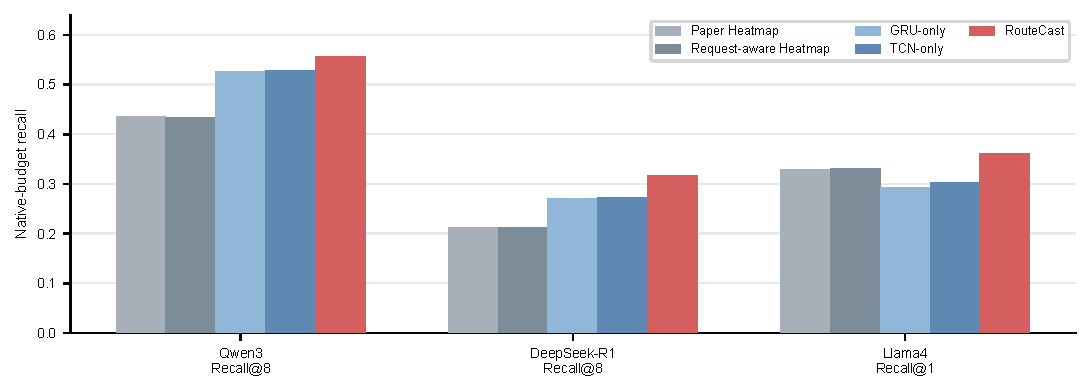
\includegraphics[width=\linewidth]{figures_final/Fig2a_MainComparison}
\end{minipage}\hfill
\begin{minipage}[c]{0.33\textwidth}
\centering
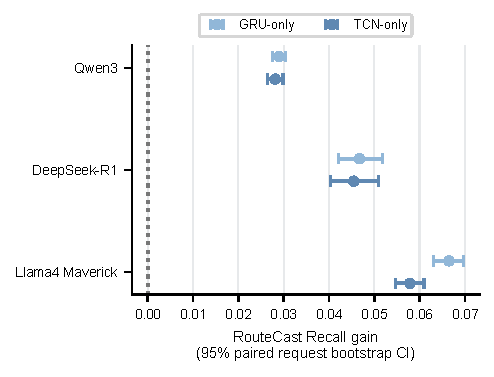
\includegraphics[width=\linewidth]{figures_final/Fig2b_RequestBootstrap}
\end{minipage}
\caption{Cross-model forecasting under the stable limit=1000 protocol. Left: native-budget Recall under matched request-disjoint splits and model-specific native $K$. Right: absolute RouteCast gains over GRU-only and TCN-only with 95\% paired request-level bootstrap intervals. RouteCast exceeds statistical, recurrent, and convolutional comparators across all three routing regimes.}
\label{fig:main}
\end{figure*}

We additionally repeated matched RouteCast and TCN training with seeds 2024, 2025, and 2026 in the limit=100 development setting. RouteCast exceeded TCN for every model under every seed. Its mean Recall advantage was $0.0317\pm0.0017$ on Qwen3, $0.0196\pm0.0062$ on DeepSeek-R1, and $0.0219\pm0.0041$ on Llama4 Maverick (mean $\pm$ sample standard deviation across seeds; Fig.~\ref{fig:tcn-seeds}). This screening supports optimization stability, while the request-level bootstrap on limit=1000 remains the primary uncertainty analysis.

\begin{table}[!t]
\centering
\caption{Native-budget limit=1000 results. Precision equals Recall at native K.}
\label{tab:main}
\scriptsize
\setlength{\tabcolsep}{2.4pt}
\begin{tabular}{llccc}
\toprule
Model & Method & Recall & MRR & NDCG \\
\midrule
Qwen3 & Heatmap & .4352 & .7969 & .4859 \\
& Request-aware & .4330 & .7956 & .4834 \\
& GRU-only & .5268 & .8893 & .5903 \\
& TCN-only & .5277 & .8902 & .5936 \\
& \textbf{RouteCast} & \textbf{.5558} & \textbf{.9013} & \textbf{.6208} \\
\midrule
DeepSeek-R1 & Heatmap & .2131 & .5087 & .2413 \\
& Request-aware & .2121 & .5076 & .2402 \\
& GRU-only & .2705 & .6715 & .3243 \\
& TCN-only & .2717 & .6707 & .3265 \\
& \textbf{RouteCast} & \textbf{.3172} & \textbf{.7131} & \textbf{.3743} \\
\midrule
Llama4 & Heatmap & .3298 & .4593 & .3298 \\
& Request-aware & .3311 & .4653 & .3311 \\
& GRU-only & .2938 & .4470 & .2938 \\
& TCN-only & .3024 & .4451 & .3024 \\
& \textbf{RouteCast} & \textbf{.3602} & \textbf{.4988} & \textbf{.3602} \\
\bottomrule
\end{tabular}
\end{table}

\subsection{Budget Expansion Reveals Model-Specific Cost}
Increasing the number of prefetched experts raised coverage for every model, but the gain came with rapidly increasing waste (Fig.~\ref{fig:budget}). For Qwen3, moving from $K=8$ to 16 increased Recall from 0.5835 to 0.7886 while waste rose from 0.4165 to 0.6057. DeepSeek-R1 remained substantially harder: Recall rose from 0.2572 to only 0.3618 and waste reached 0.8191 at $K=16$. For Llama4, increasing $K$ from 1 to 8 raised Recall from 0.2848 to 0.6540, but 91.8\% of prefetched experts were false positives. These curves rule out ``prefetch more'' as a sufficient solution and motivate calibrated selection and abstention.

\begin{figure*}[!t]
\centering
\begin{minipage}[c]{0.67\textwidth}
\centering
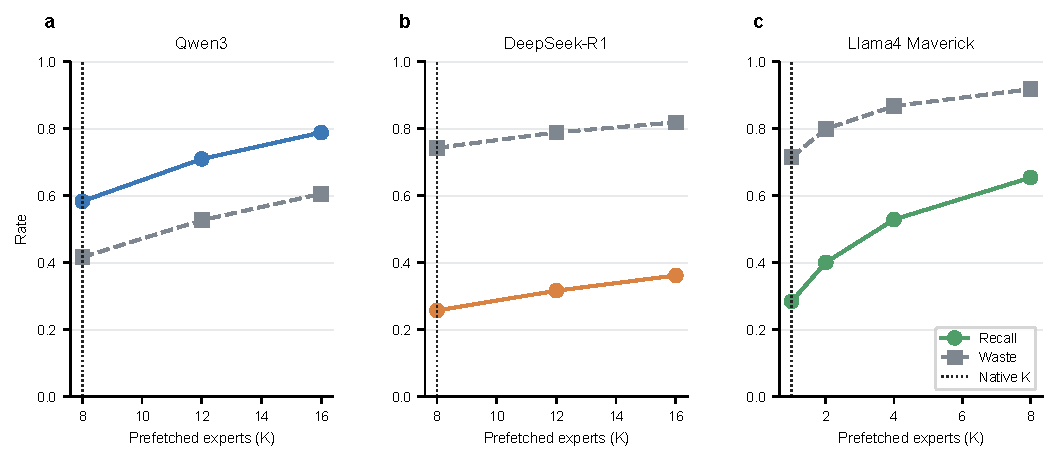
\includegraphics[width=\linewidth]{figures_final/Fig3_BudgetTradeoff}
\end{minipage}\hfill
\begin{minipage}[c]{0.30\textwidth}
\centering
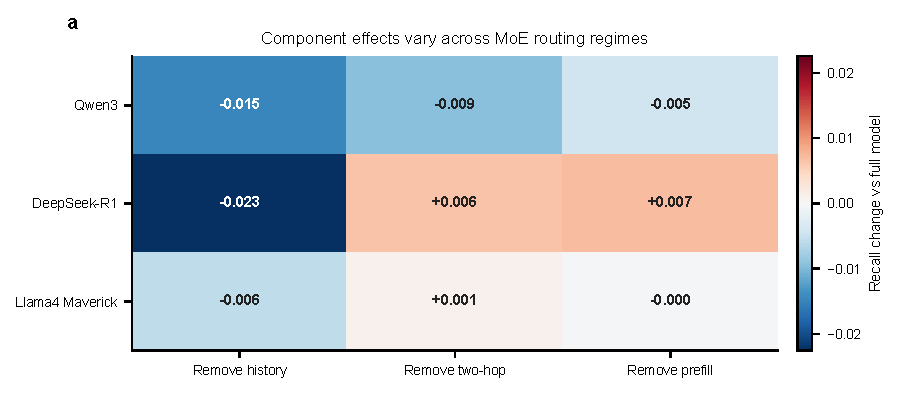
\includegraphics[width=\linewidth]{figures_final/Fig4_ComponentAblation}
\end{minipage}
\caption{Why fixed-width prediction is insufficient. Left: budget--quality trade-offs across the three routing regimes; dotted lines mark native $K$. Right: native-budget Recall change after removing route-evidence components. Wider candidate sets increase coverage but also waste, while branch utility varies by routing regime.}
\label{fig:budget}
\label{fig:ablation}
\end{figure*}

\subsection{Component Utility Depends on the Routing Regime}
Cross-token history was the only ablated component whose removal degraded all three models (Fig.~\ref{fig:ablation}). Removing it reduced Recall by 0.0148 on Qwen3, 0.0226 on DeepSeek-R1 and 0.0056 on Llama4. Two-hop and prefill features helped Qwen3 but were neutral or harmful for the other families. In particular, removing two-hop or prefill evidence improved DeepSeek-R1 by approximately 0.0064 and 0.0069. The result supports conditional fusion rather than the stronger claim that every branch is universally beneficial.

\subsection{Calibration Enables Adaptive Candidate Selection}
Temperature scaling served two distinct purposes. First, it measured whether the score magnitude represented expert-membership confidence. Second, it controlled how quickly the categorical probability accumulated and therefore how many candidates satisfied Eq.~\eqref{eq:mass-selection}. Since temperature does not alter score order, any change in dynamic width comes from probability concentration rather than improved ranking.

The fitted temperatures differed sharply across models: 0.82 for Qwen3, 0.32 for DeepSeek-R1, and 1.05 for Llama4 Maverick. Figure~\ref{fig:calibration-budget}a shows the corresponding test ECE. Scaling reduced ECE from 0.2894 to 0.2801 on Qwen3 and from 0.3827 to 0.2763 on DeepSeek-R1. For Llama4 Maverick, ECE changed from 0.1236 to 0.1250, a slight deterioration. Thus, temperature scaling substantially corrected DeepSeek-R1 confidence but did not improve every model. The low DeepSeek-R1 temperature indicates that its logits required sharpening; it does not imply higher forecasting accuracy.

Validation then selected masses of 0.70, 0.95, and 0.50 for Qwen3, DeepSeek-R1, and Llama4 Maverick, respectively (Fig.~\ref{fig:calibration-budget}b). These choices produced average candidate widths of 11.75, 17.25, and 6.56, with validation Recall of 0.6120, 0.3786, and 0.6293. DeepSeek-R1 therefore required both the highest cumulative mass and the widest candidate set, yet achieved the lowest Recall. This result identifies a routing-regime limitation rather than a calibration failure: reshaping confidence cannot recover information absent from the route history. The model-specific operating points also rule out one global mass threshold as a reliable cross-architecture policy.

\begin{figure}[!t]
\centering
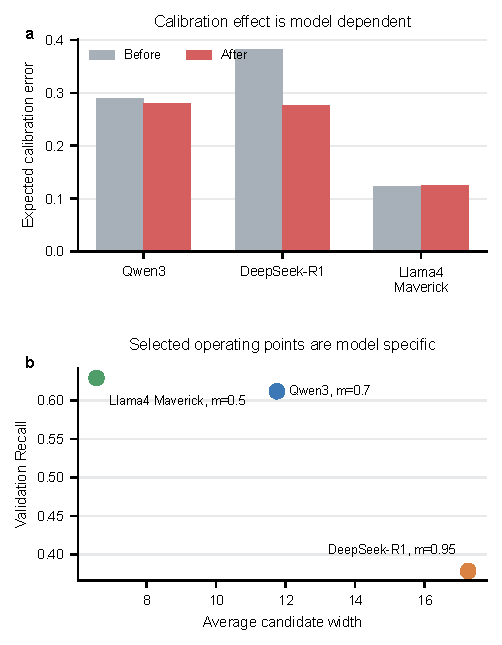
\includegraphics[width=0.96\columnwidth]{figures_final/Fig5_CalibrationSelection}
\caption{Calibration and adaptive-budget selection. (a) Test expected calibration error before and after per-model temperature scaling. Lower is better. Scaling strongly improves DeepSeek-R1, modestly improves Qwen3, and slightly worsens Llama4 Maverick. (b) Validation-selected operating points. Labels report cumulative mass; coordinates show the resulting average candidate width and Recall. Full reliability diagrams and mass sweeps are provided in the supplementary figure package.}
\label{fig:calibration-budget}
\end{figure}

\subsection{Selective Scheduling Changes Cache-Replay Outcomes}
Prediction Recall does not determine cache utility because resident candidates require no transfer, wrong candidates can evict useful experts, and the same prediction budget has different consequences at different capacities. Figure~\ref{fig:cache-pareto} therefore plots cache hit rate against total expert transfers rather than reporting either quantity alone. Movement toward the upper-left indicates a better operating point.

On Qwen3, the adaptive-cache policy achieved hit rates of 0.5345, 0.7197, and 0.8771 at capacities $1\times$, $2\times$, and $4\times$, requiring 1.00, 0.62, and 0.31 million transfers (Fig.~\ref{fig:cache-pareto}a). Relative to unfiltered adaptive mass, cache-aware rejection reduced transfers by 53--62\%. At $4\times$ capacity it retained nearly the same hit rate, 0.8771 versus 0.8775, while avoiding roughly 0.10 million transfers. At $1\times$, however, fixed native prefetching achieved a higher hit rate with only moderately more transfers, showing that aggressive rejection can discard useful predictions when capacity is tight.

DeepSeek-R1 displayed the clearest failure boundary (Fig.~\ref{fig:cache-pareto}b). Fixed native prefetching achieved the highest hit rate at every tested capacity. The adaptive-cache policy reduced transfers relative to adaptive mass but did not recover the lost hit rate. This outcome is consistent with DeepSeek-R1's lower forecasting Recall: selective admission can suppress waste, but it cannot make weak candidates informative.

Llama4 Maverick showed a different trade-off (Fig.~\ref{fig:cache-pareto}c). Adaptive cache achieved the highest hit rate at $2\times$ and $4\times$ capacity while using far fewer transfers than adaptive mass. Nevertheless, LRU remained cheaper in transfer count. The benefit is therefore conditional: selective prefetching improves residency quality when additional movement is acceptable, but it does not dominate demand-only caching on both axes.

\begin{figure}[!t]
\centering
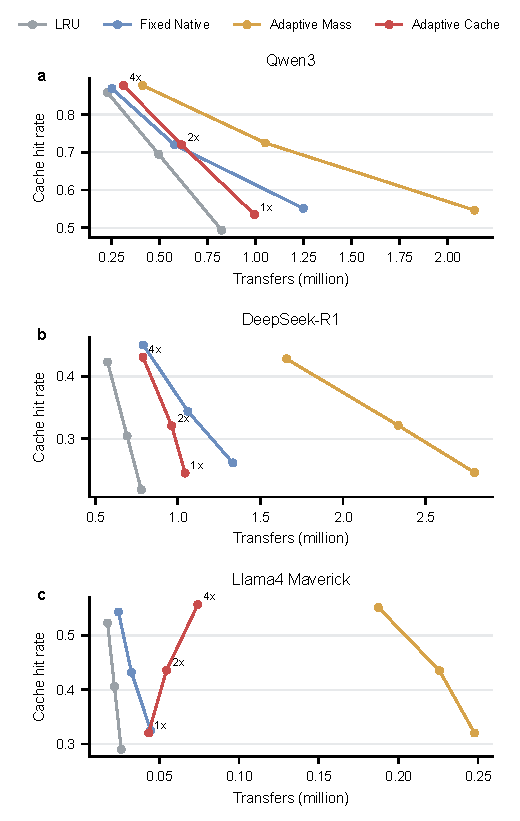
\includegraphics[width=0.96\columnwidth]{figures_final/Fig6_CachePareto}
\caption{Trace-driven cache Pareto analysis for (a) Qwen3, (b) DeepSeek-R1, and (c) Llama4 Maverick. Each curve contains cache capacities of $1\times$, $2\times$, and $4\times$; labels identify the adaptive-cache points. Upper-left movement is preferable because it combines higher hit rate with fewer transfers. Cache-aware rejection consistently reduces transfers relative to unfiltered adaptive mass, but the best policy depends on model and capacity.}
\label{fig:cache-pareto}
\end{figure}

\FloatBarrier

\section{Discussion}
Discrete route histories retained predictive information across all three evaluated MoE families. TCN-only slightly improved over GRU-only in native-budget Recall, confirming that dilated temporal convolutions form a competitive history encoder. RouteCast nevertheless exceeded both models with paired confidence intervals above zero. The improvement therefore depends on more than the choice of recurrent or convolutional sequence encoder. Statistical priors stabilized sparse observations, temporal features captured recent deviations, and the gate adapted their contribution to context. No individual evidence branch was universally beneficial.

Forecasting quality and prefetch utility must nevertheless be evaluated separately. Wider candidate sets increased Recall but were particularly inefficient for DeepSeek-R1 and Top-1 Llama4 Maverick. Calibration made candidate scores comparable within each model. Rejection and cache-aware admission then determined whether a candidate justified speculative movement. Cache replay shows that this separation limits transfer amplification, but it does not guarantee universal system gains.

Three limitations bound these conclusions. First, public traces cannot measure transfer--compute overlap, exposed stalls, throughput, energy, or kernel overhead. Second, most scheduling and cache ablations use the limit=100 development setting; limit=1000 evidence currently covers the forecaster and primary baselines. Third, the learned comparators now include matched GRU and TCN models, but not a matched transformer. Limit=1000 multi-seed training and a current overhead benchmark remain necessary for a stronger systems claim.

\section{Conclusion}
RouteCast combines calibrated next-token expert forecasting with selective cache-aware prefetching. Under request-disjoint evaluation, it improved native-budget Recall, MRR, and NDCG across Qwen3, DeepSeek-R1, and Llama4 Maverick traces. Calibration and adaptive selection exposed the trade-off between coverage and speculative movement. Cache replay identified both transfer reductions and model-specific failure regions. These results support RouteCast as an algorithmic interface between forecasting and cache management, while end-to-end acceleration remains unverified.

\appendix
\section{Additional Evidence}
The accompanying supplementary figure package contains dataset composition, development-stage history sensitivity, limit=100 versus limit=1000 scale comparison, three-seed screening, legacy layer heterogeneity, calibration metrics, a legacy gate-overhead benchmark and the complete cache-replay tables. Legacy Qwen-only panels are labelled explicitly and are not used as evidence for the cross-model RouteCast V3 claim. The former 3-by-3 cache matrix is supplied separately rather than embedded as an unreadable composite figure.

\begin{figure}[!t]
\centering
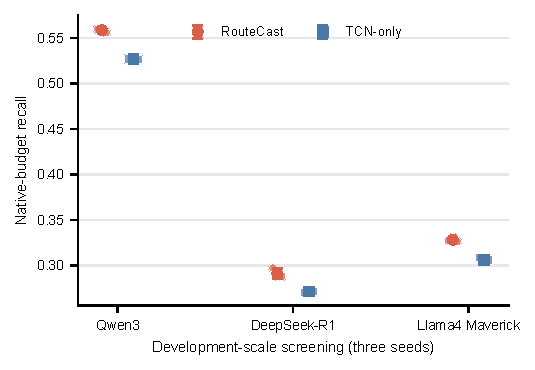
\includegraphics[width=0.95\columnwidth]{figures_final/FigS1_SeedStability}
\caption{Development-scale stability screening over seeds 2024, 2025, and 2026. Small translucent points denote individual runs; large markers and error bars denote mean $\pm$ sample standard deviation. RouteCast exceeds the matched TCN-only baseline for all nine model--seed pairs.}
\label{fig:tcn-seeds}
\end{figure}

\begin{thebibliography}{00}
\bibitem{pregated} R. Hwang et al., ``Pre-gated MoE: An algorithm-system co-design for fast and scalable mixture-of-expert inference,'' in \emph{Proc. ISCA}, 2024.
\bibitem{moeinfinity} L. Xue et al., ``MoE-Infinity: Efficient MoE inference on personal machines with sparsity-aware expert cache,'' arXiv:2401.14361, 2024.
\bibitem{promoe} X. Song et al., ``ProMoE: Fast MoE-based LLM serving using proactive caching,'' arXiv:2410.22134, 2024.
\bibitem{patterns} Z. Yu et al., ``Patterns behind chaos: Forecasting data movement for efficient large-scale MoE LLM inference,'' arXiv:2510.05497, 2026.
\bibitem{specmd} D. Hoang et al., ``SpecMD: A comprehensive study on speculative expert prefetching,'' arXiv:2602.03921, 2026.
\bibitem{stmoe} Y. Zhao et al., ``A spatio-temporal expert prefetching framework for efficient MoE-based LLM inference,'' arXiv:2606.15453, 2026.
\bibitem{specprefetch} J. Kong et al., ``SpecPrefetch: Parameter-efficient expert prefetching for sparse MoE foundation models,'' arXiv:2607.24787, 2026.
\end{thebibliography}

\end{document}
